%-----------------------------------------------------------------------------
%	PACKAGES AND DOCUMENT CONFIGURATIONS
%-----------------------------------------------------------------------------

\documentclass{article}

\usepackage{graphicx} % Required for the inclusion of images
\usepackage{natbib} % Required to change bibliography style to APA
\usepackage{amsmath} % Required for some math elements
\usepackage{amssymb}
\usepackage{grffile}
\usepackage[export]{adjustbox}
\usepackage{subcaption}
\usepackage{float}
\usepackage{listings}
\usepackage[margin=1.0in]{geometry}
\usepackage{tikz}
\usepackage{enumitem}
\usepackage{scrextend}
\usepackage{siunitx}
\usepackage{minted}
\usepackage{listings}

\usetikzlibrary{shapes.geometric, arrows}
\tikzstyle{startstop} = [rectangle, rounded corners, minimum width=1cm, minimum height=1cm,text centered, draw=black, fill=white!30]
\tikzstyle{process} = [rectangle, minimum width=1.5cm, minimum height=1cm, text centered, draw=black, fill=white!30]
\tikzstyle{arrow} = [thick,<->,>=stealth]

\renewcommand{\baselinestretch}{1.5}
\setlength{\parskip}{1em}
\setlength\parindent{0pt} % Removes all indentation from paragraphs

%-----------------------------------------------------------------------------
%	DOCUMENT INFORMATION
%-----------------------------------------------------------------------------

\title{ECE 547 Project 2} % Title

\author{Yang \textsc{Wang}}  % Author name

\date{\today} % Date for the report

\begin{document}

\maketitle % Insert the title, author and date

%-----------------------------------------------------------------------------
%	Problems
%-----------------------------------------------------------------------------

\section*{Part 1}
	For extracting the time and the sequence number of each TCP data sent and each
	acknowledgement received at node $n_{0}$. We need to look into
	\emph{tcp-window.tr} to search for the needed information.

	\emph{tcp-window.tr} is a space-seperated file which each column corresponds
	to some information. By using this reference [1], we are able to parse out
	what each column represents: the first column is the event. The second is the
	time and the 13th is the sequence number.

	For extracting the sequence number of each TCP data packet sent, we need to
	look for ``+'' along with the keyword ``tcp'' for each line in the trace file.
	For extracting the sequence number of each acknowledgement received, we need
	to look for ``r'' along with the keyword ``ac'' for each line.
	
	This combination of Shell command is used for extracting the needed
	information:
	\begin{minted}{shell}
		cat tcp-window.tr | grep "+.*tcp" | cut -f2,11 -d " " > tcp\_seqnum
		cat tcp-window.tr | grep "r.*ack" | cut -f2,11 -d " " > ack\_seqnum
	\end{minted}
	
	This MATLAB script is used to plot the figure for part 1:
	\inputminted[tabsize=2,breaklines]{matlab}{proj1\_p1.m}

	The corresponding figure is shown in Figure 1 in Appendix.

\section*{Part 2}
	For extracting the congestion window size (\emph{cwnd}), we need to look into
	\emph{tcp-window.nam} file to search for the needed information.

	The variable trace is already enabled in \emph{tcp-window.tcl} script. Hence,
	we only need to look for any line in the \emph{tcp-window.nam} that matches
	with the keyword ``cwnd\_''.

	This combination of Shell command is used for extracting the needed
	information:
	\begin{minted}{shell}
		cat tcp-window.nam | grep "cwnd\_" | cut -f3,13 -d " " > cwnd
	\end{minted}
	
	This MATLAB script is used to plot the figure for part 1:
	\inputminted[tabsize=2,breaklines]{matlab}{proj1\_p2.m}

	The corresponding figure is shown in Figure 2 in Appendix.

\section*{Part 3}
	From Figure 1, the slow start phase of the TCP flow ended at approximately
	2.3 second when the \emph{cwnd} almost hit 30. There are 7 congestion
	avoidance phases. Here are the rough estimates in seconds: 5 to 8, 10 to 14,
	16 to 20, 22 to 26, 27 to 32, 33 to 36 and 37 to 40.

\section*{Part 4}
	Using the same scripts in Part 1 and 2. We can generate the same plots for TCP
	Reno agent. The plots are shown as Figure 3 and 4 in Appendix.

	The MATLAB scripts are listed below:
	\inputminted[tabsize=2,breaklines]{matlab}{proj1\_p3.m}
	\inputminted[tabsize=2,breaklines]{matlab}{proj1\_p4.m}

	For TCP Reno, although it is little difficult to see from Figure 3, we know
	that that fast retransmit and recovery occurs when the sender receives 3
	duplicate ACKs. Hence, the fast restransmit and recovery phases can be
	identified roughly at 2.7, 8.2, 13.2, 17.5, 22.5, 27.5, 32.5 and 36.5 seconds.
	\pagebreak

\section*{Appendix}
	\begin{figure}[!hbt]
		\centering
		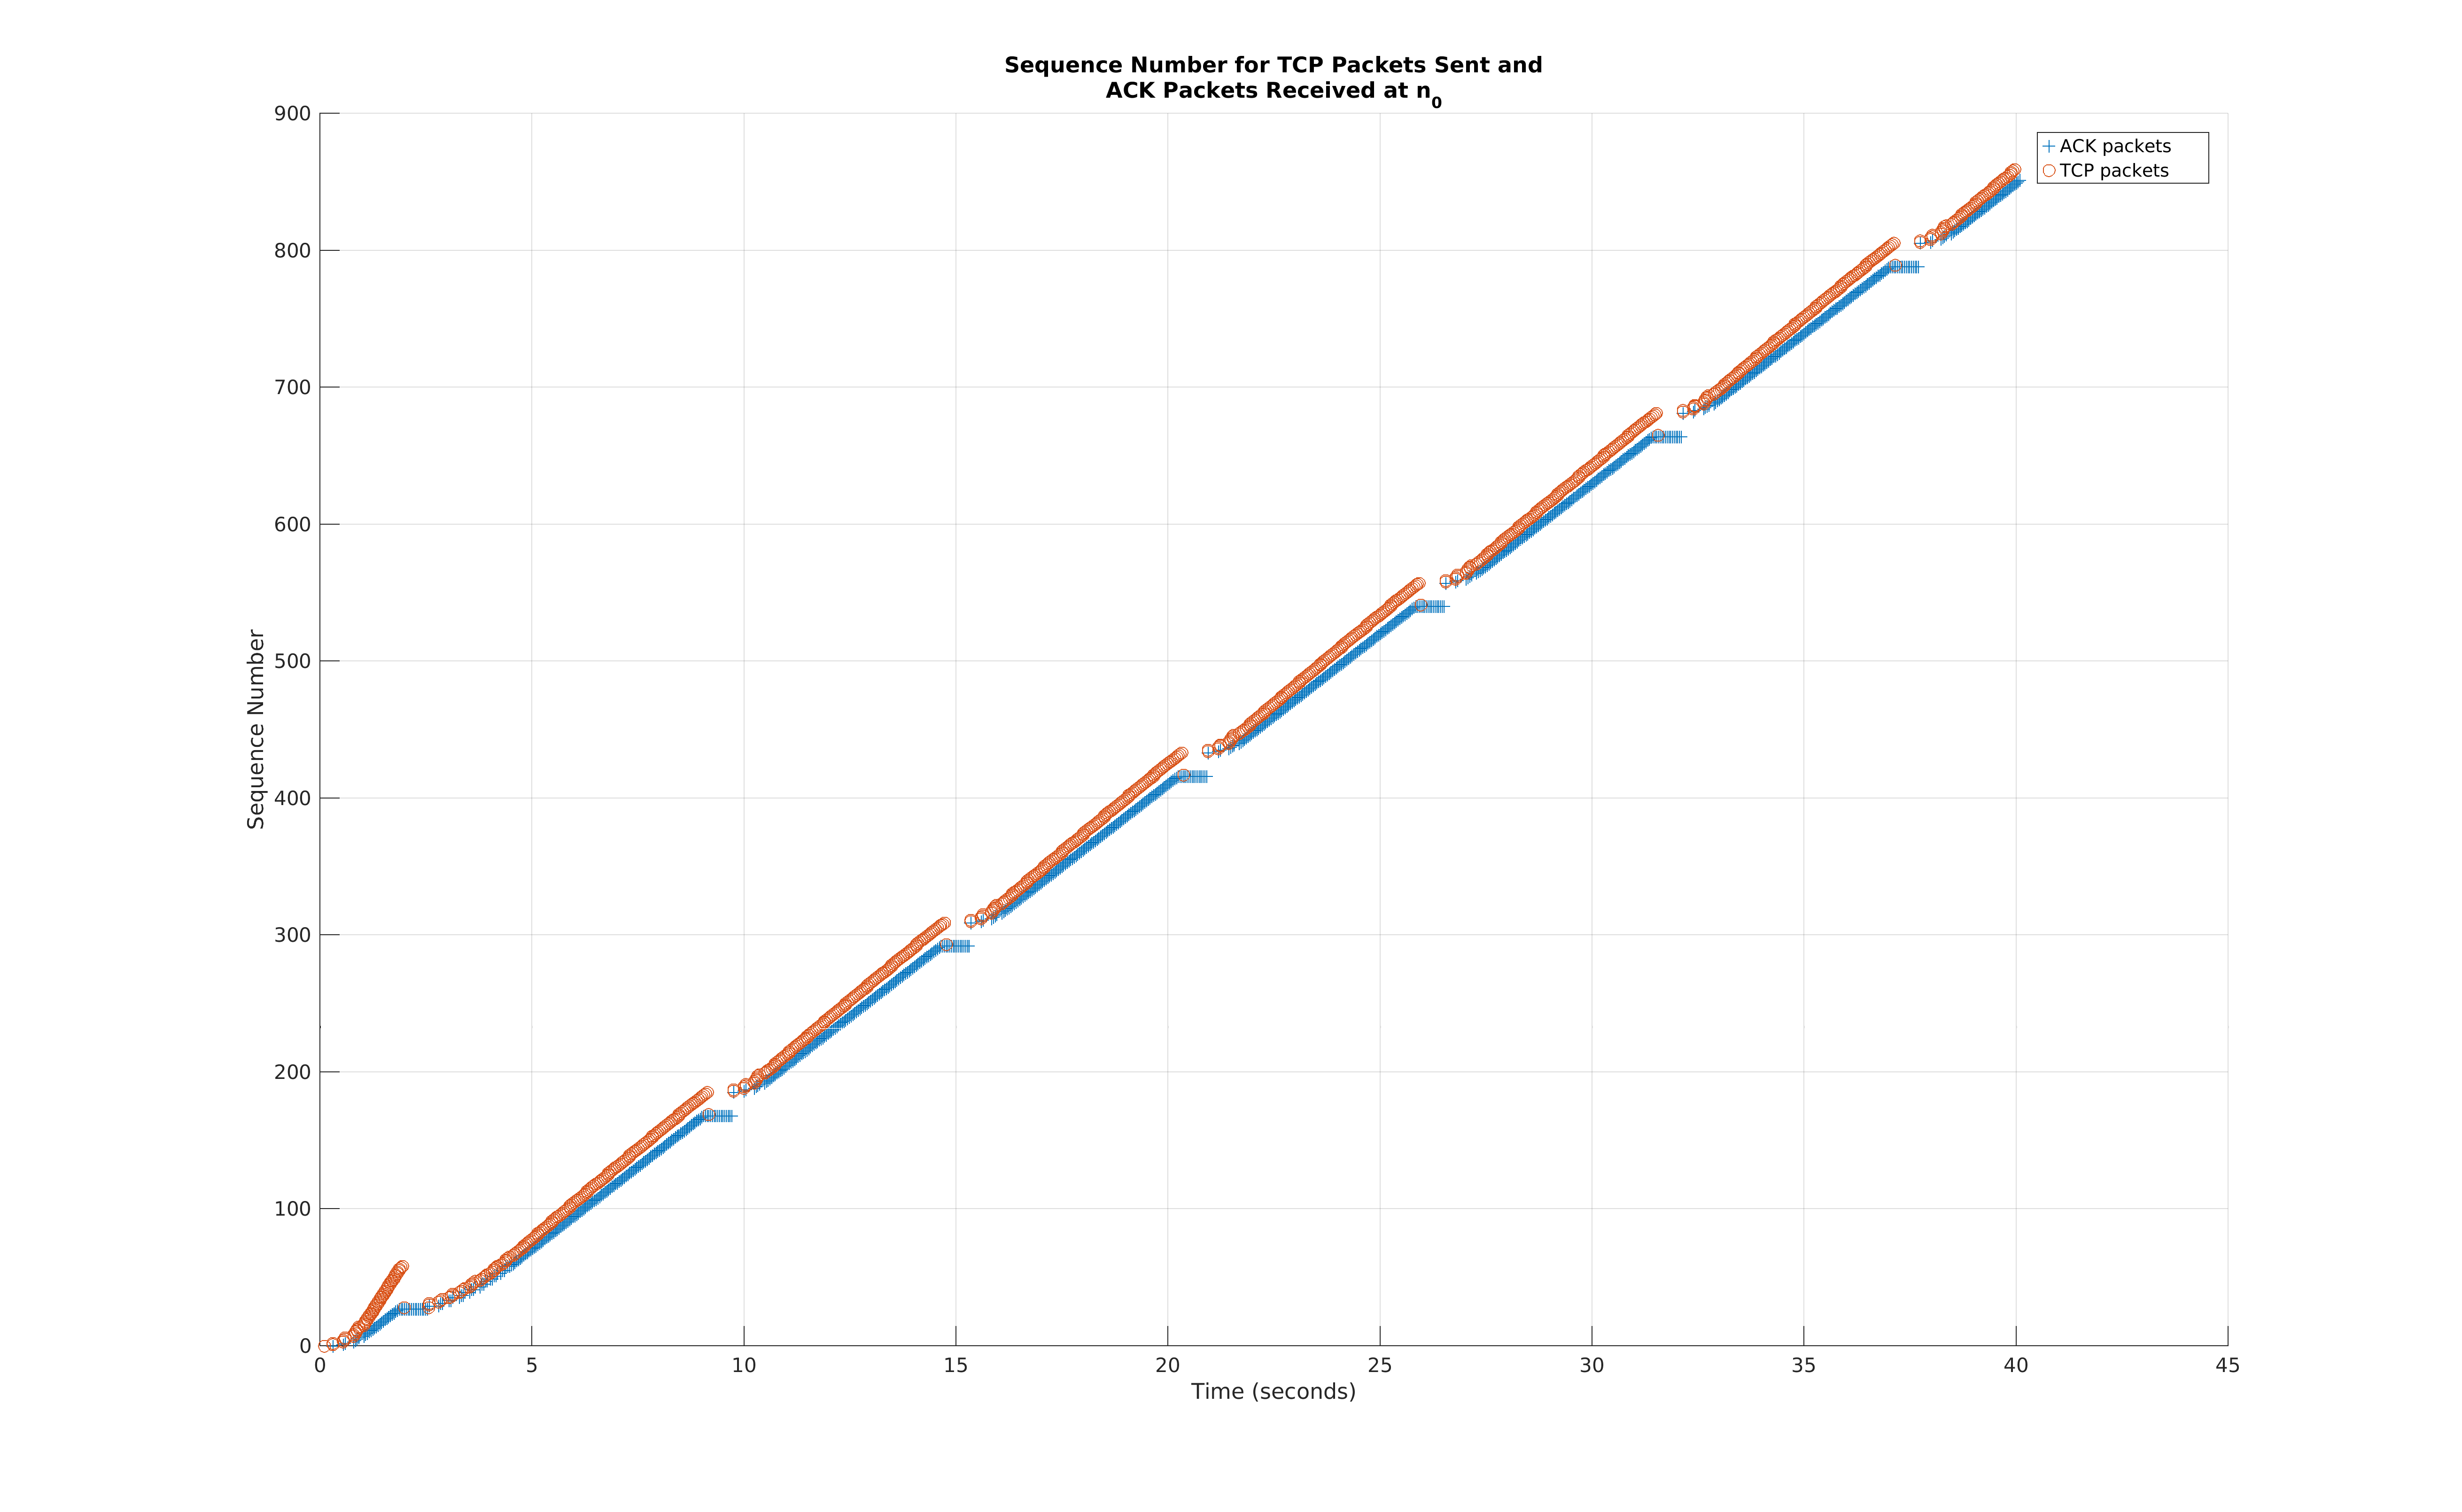
\includegraphics[width=0.85\linewidth]{proj2_p1.png}
		\caption{Sequence number vs. time.}
	\end{figure}

	\begin{figure}[!hbt]
		\centering
		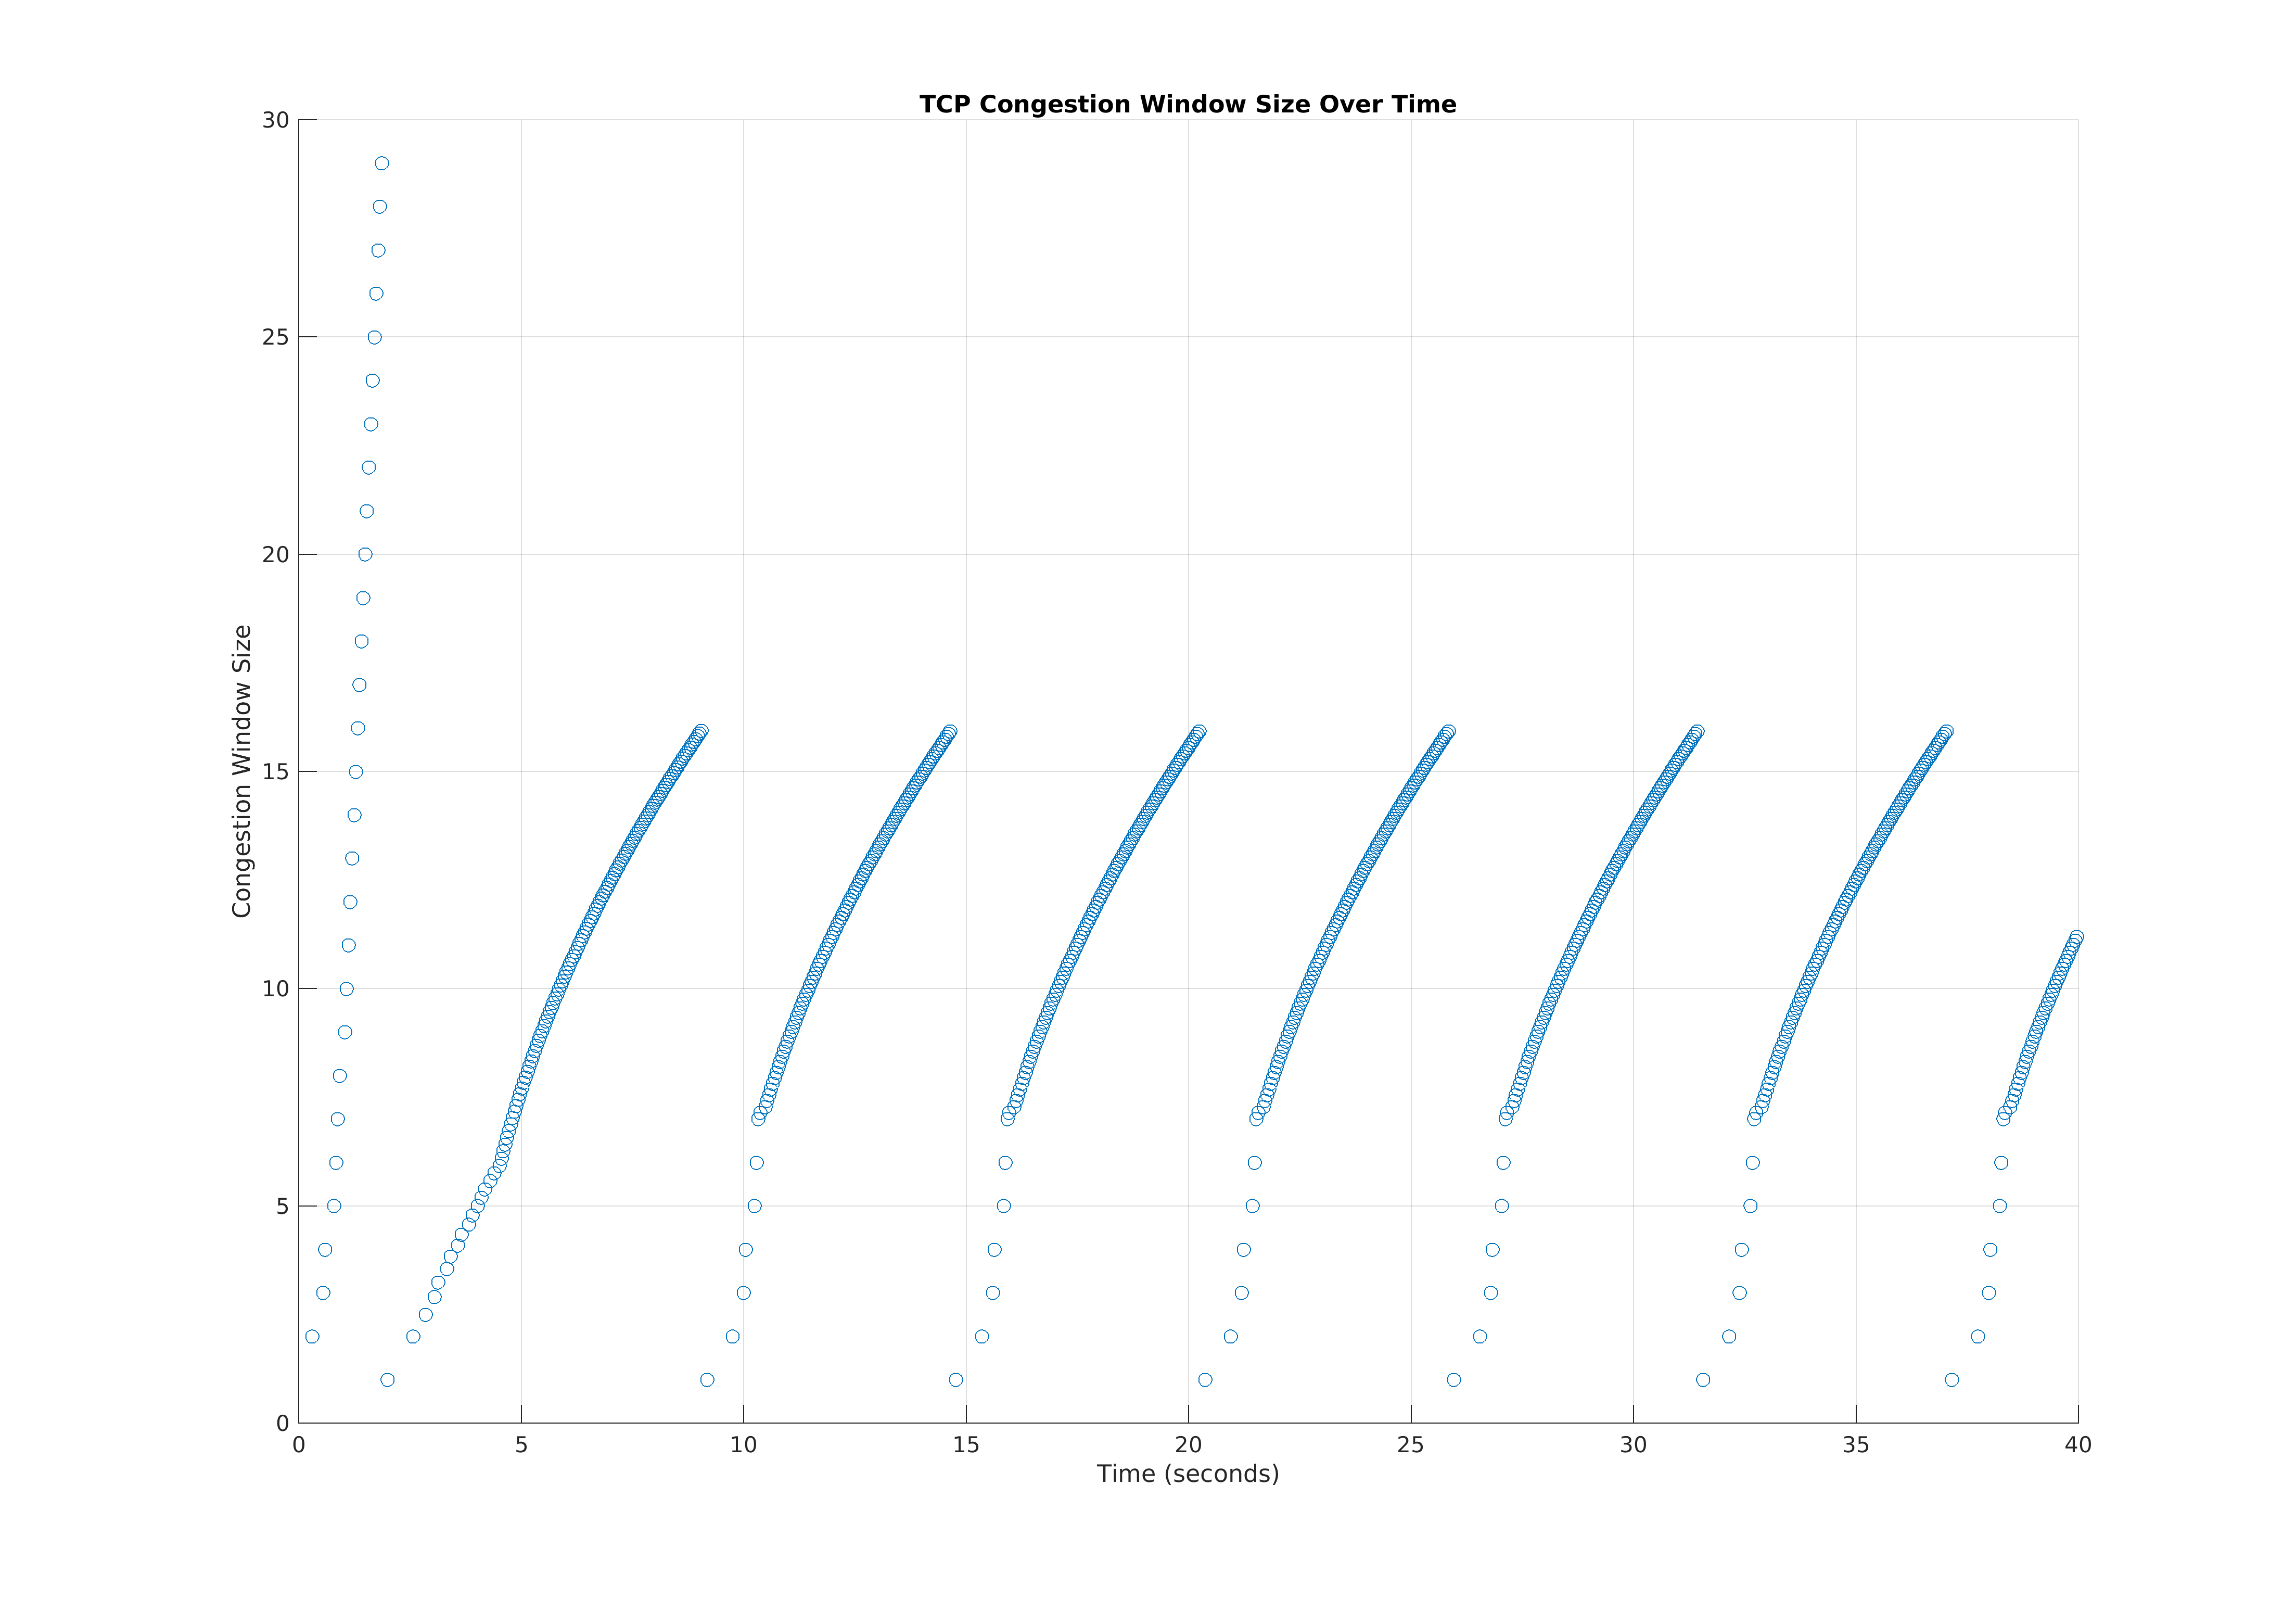
\includegraphics[width=0.85\linewidth]{proj2_p2.png}
		\caption{Congestion window size vs. time.}
	\end{figure}

	\begin{figure}[!hbt]
		\centering
		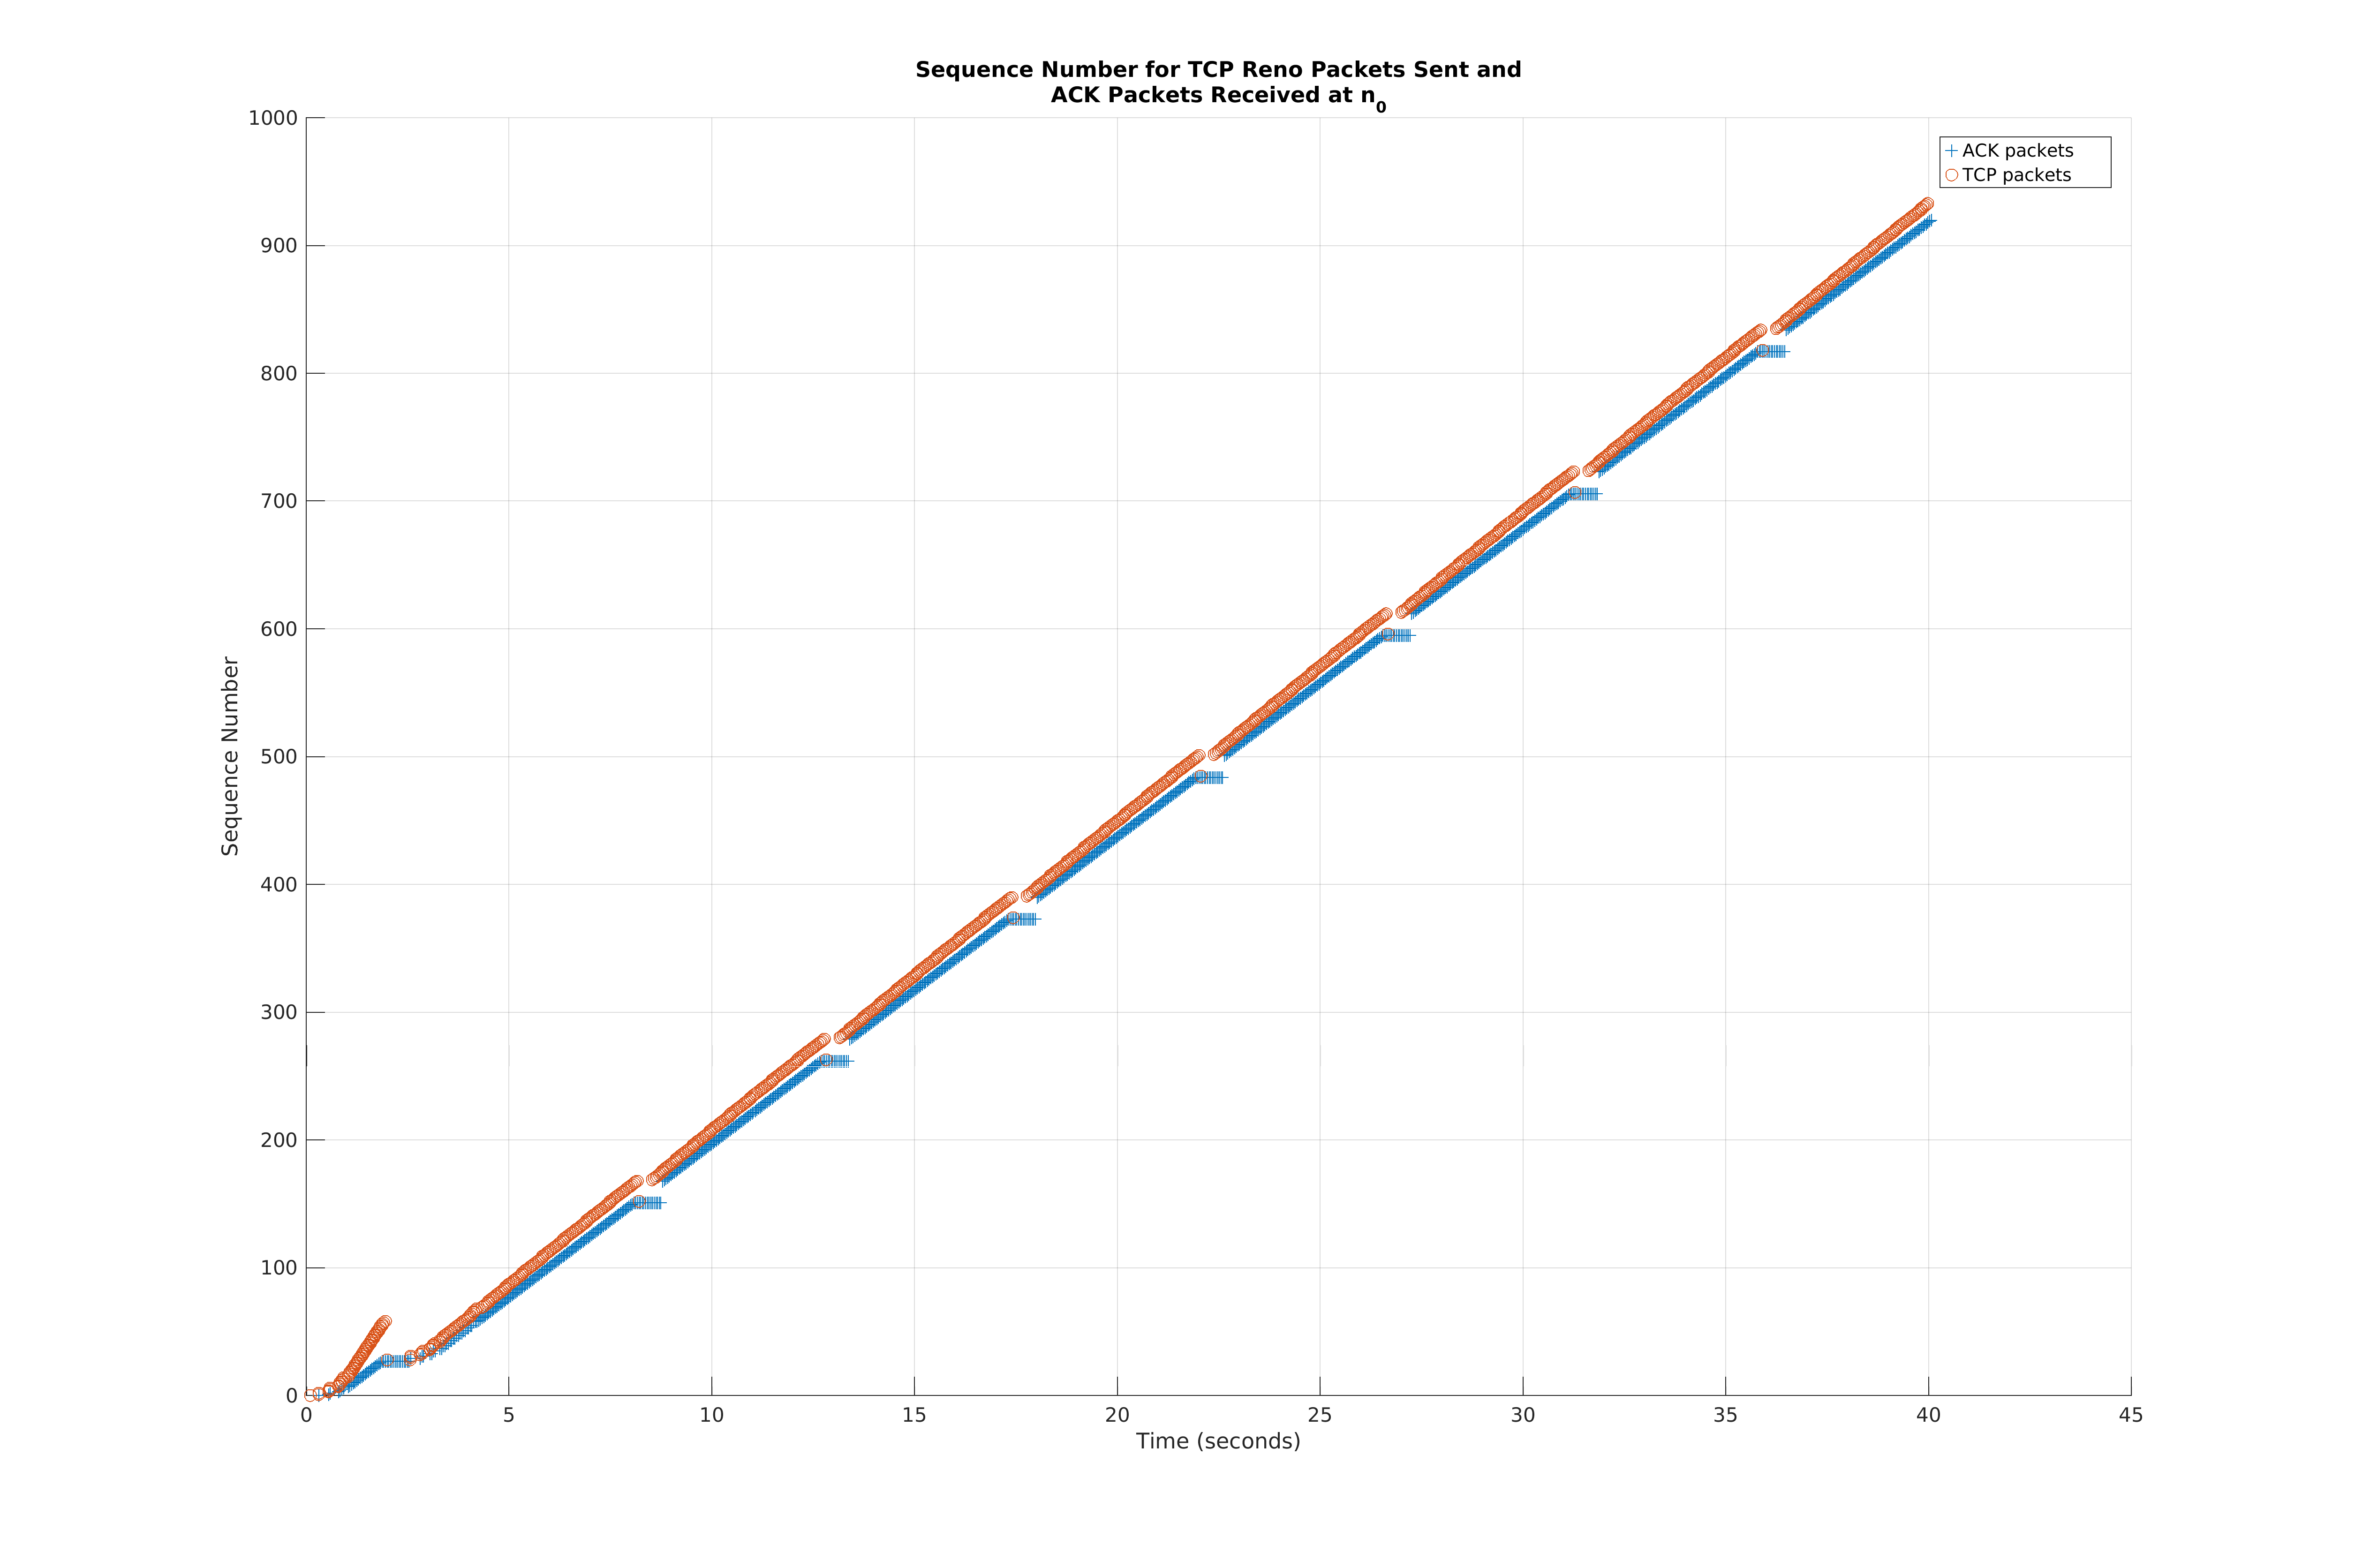
\includegraphics[width=0.85\linewidth]{proj2_p3.png}
		\caption{Sequence number vs. time (Reno).}
	\end{figure}

	\begin{figure}[!hbt]
		\centering
		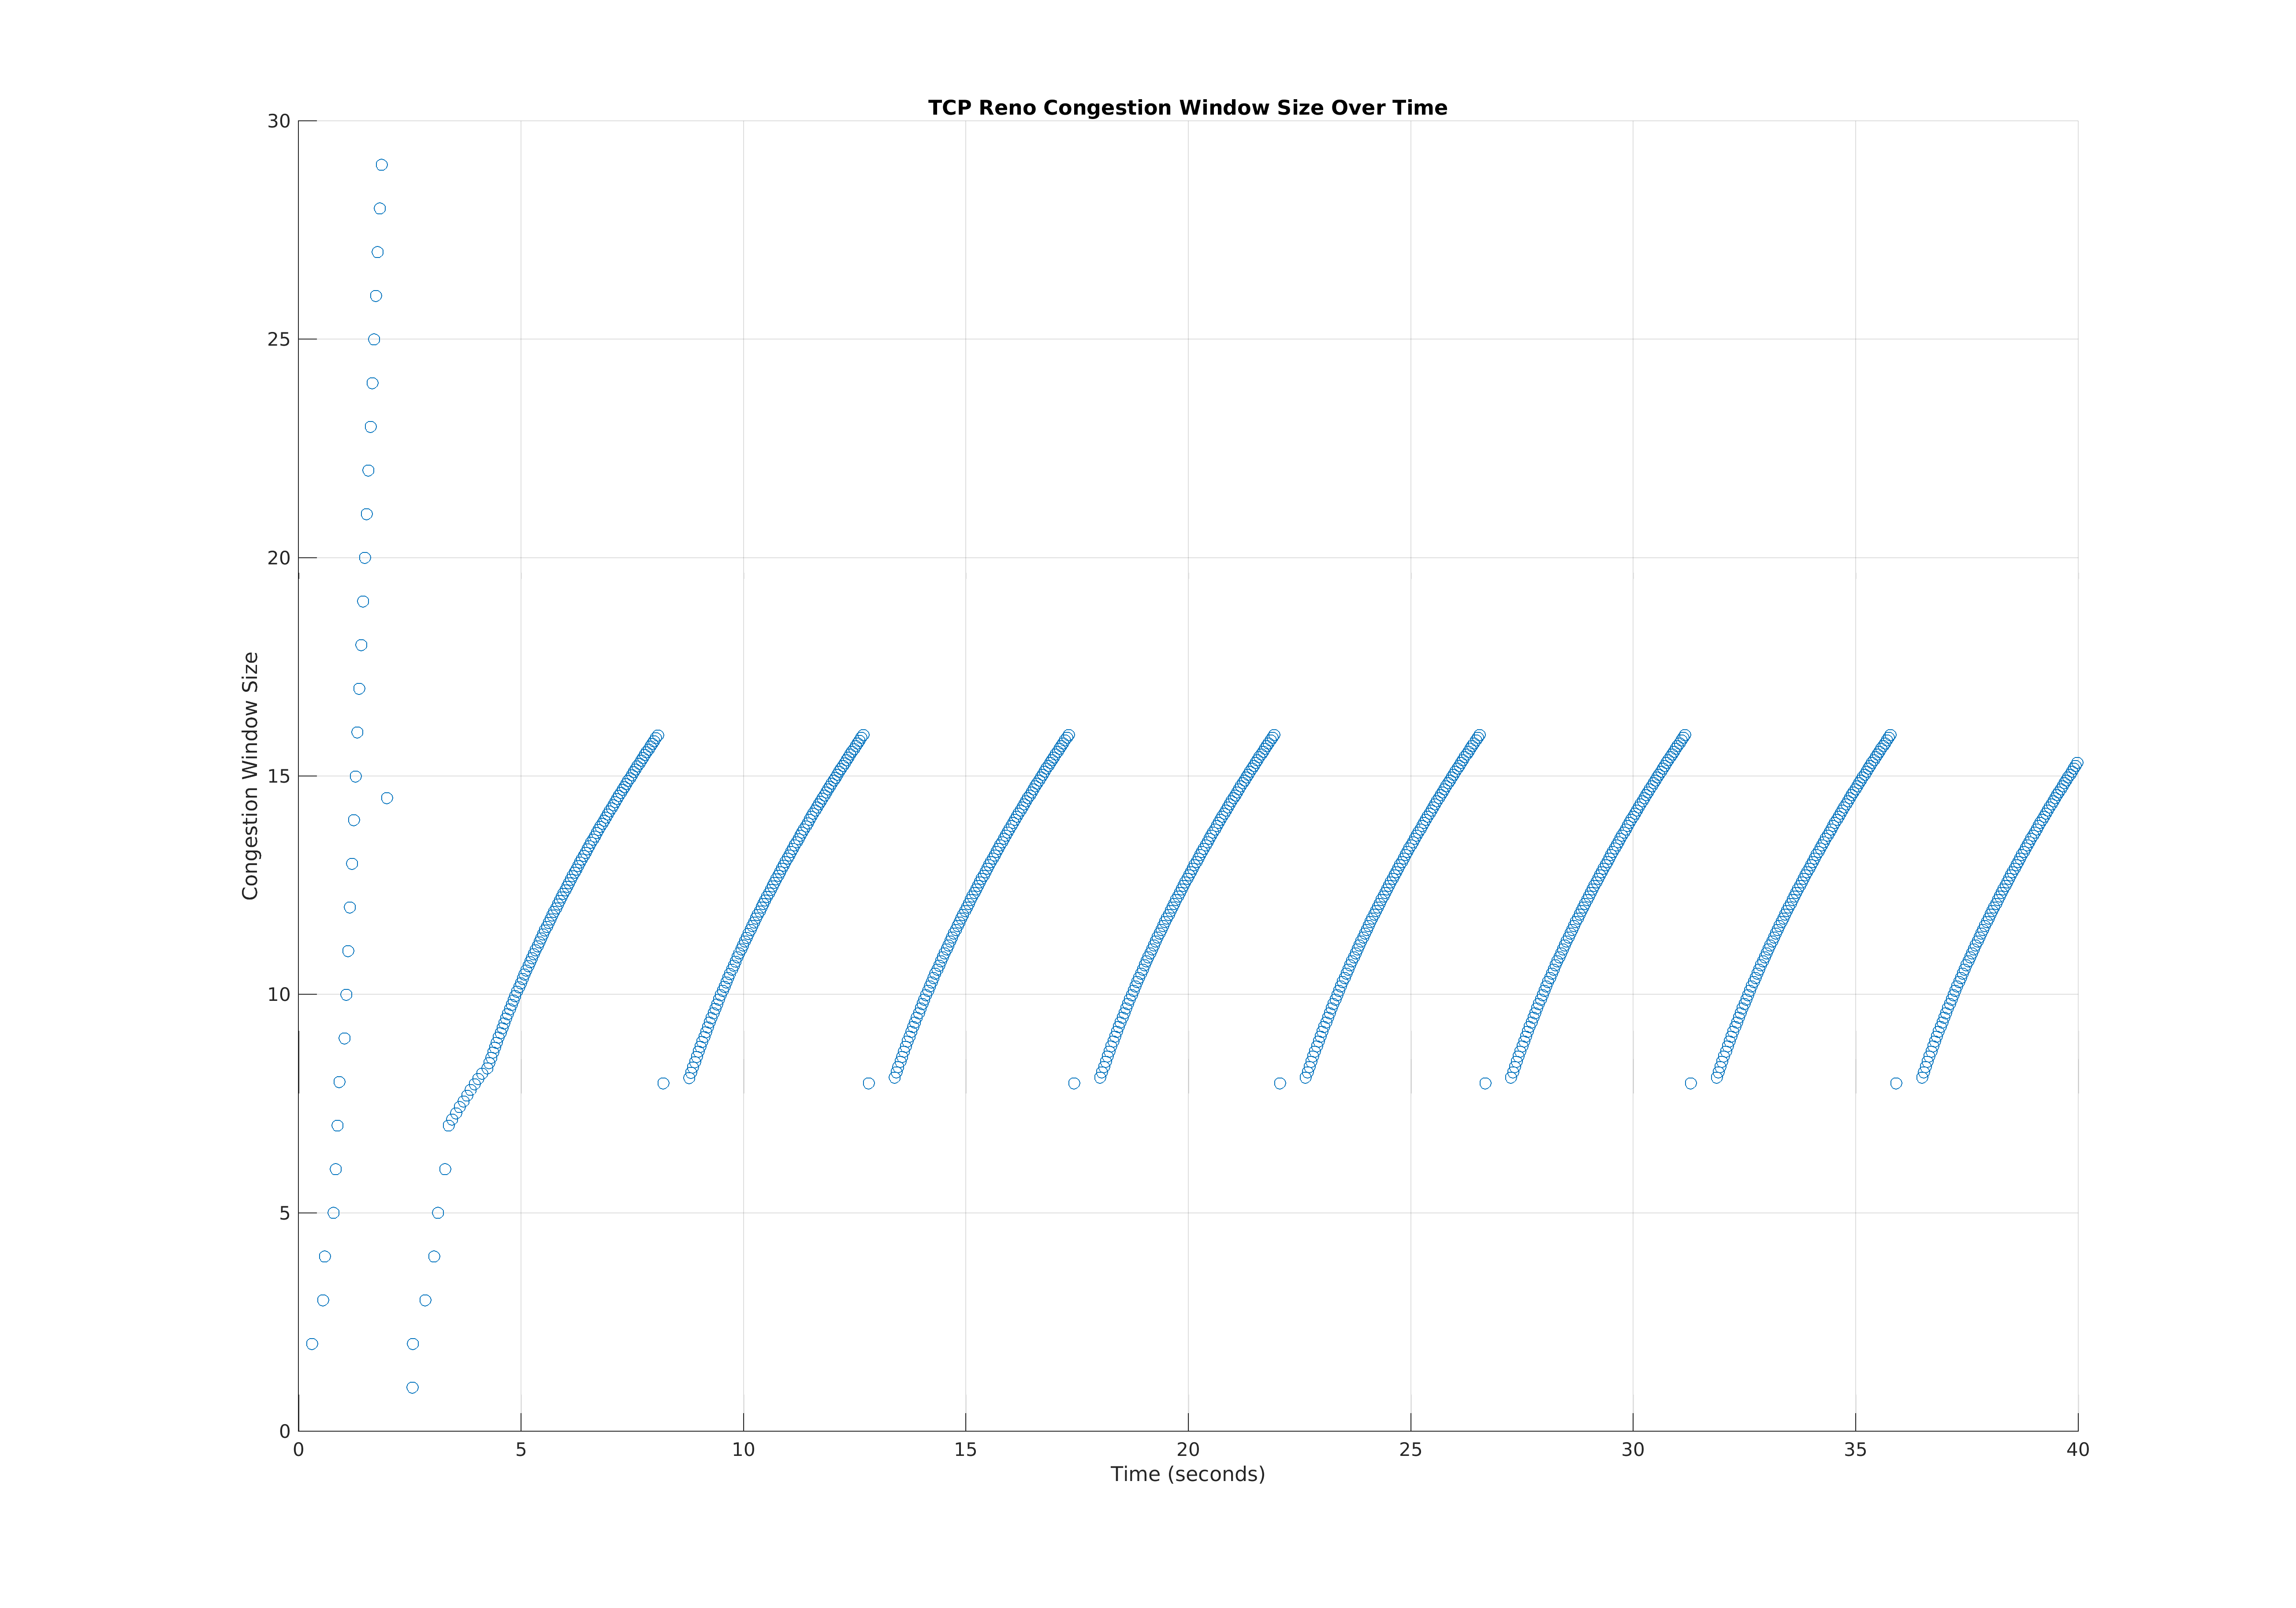
\includegraphics[width=0.85\linewidth]{proj2_p4.png}
		\caption{Congestion window size vs. time (Reno).}
	\end{figure}

\section*{Reference}

	[1] J. Chung and M. Claypool, "Trace Analysis Example," in NS by Example.
	[Online].

	Available: http://nile.wpi.edu/NS/analysis.html. Accessed: Nov. 27, 2016.

\end{document}
